\documentclass[conference]{IEEEtran}
\usepackage[T1]{fontenc}
\usepackage{amsmath,amssymb,booktabs}
\usepackage{graphicx}
\usepackage[hidelinks]{hyperref}
\setcounter{dbltopnumber}{2}
\renewcommand{\dbltopfraction}{.82}
\setlength{\dbltextfloatsep}{10pt plus 2pt minus 2pt}
\hypersetup{pdftitle={When Does Timing Feedback Help Budgeted GPU Kernel Autotuning?}}
\newcommand{\GraphRidgeDelta}{+0.07}
\newcommand{\GraphRidgeCI}{[-0.32,+0.46]}
\newcommand{\GraphColdDelta}{+8.93}
\newcommand{\GraphColdCI}{[+7.25,+10.58]}
\newcommand{\GraphNoFeedbackDelta}{+8.28}
\newcommand{\GraphNoFeedbackCI}{[+6.76,+9.78]}
\newcommand{\GraphBudgetCI}{[-1,+2]}
\newcommand{\GraphOffsetMAPE}{20.6}
\newcommand{\GraphOffsetCI}{[-3.07,-2.48]}
\newcommand{\LaunchRidgeDelta}{-0.17}
\newcommand{\LaunchRidgeCI}{[-0.45,+0.10]}
\newcommand{\LaunchColdDelta}{+0.19}
\newcommand{\LaunchColdCI}{[-1.56,+1.98]}
\newcommand{\LaunchNoFeedbackDelta}{+0.35}
\newcommand{\LaunchNoFeedbackCI}{[-0.81,+1.51]}
\newcommand{\LaunchBudgetCI}{[-1,+1]}
\newcommand{\LaunchOffsetMAPE}{25.2}
\newcommand{\LaunchOffsetCI}{[+0.35,+0.90]}


\title{When Does Timing Feedback Help Budgeted GPU Kernel Autotuning?}
\author{\IEEEauthorblockN{Author names pending}\IEEEauthorblockA{Affiliations pending}}
\begin{document}
\maketitle

\begin{abstract}
Should a GPU tuner choose four candidates in advance or wait for each
timing before choosing the next? We replay both strategies on seven
Triton kernel families across five GPU environments. We select on one
timing pass and score on another. On CUDA graph replay, a Gaussian
world model surrogate selects a configuration within 5\% of the best
with 87.9\% macro-averaged success, versus 80.7\% for a fixed portfolio
trained on similar source shapes. Supplying measured values to the
same acquisition policy raises success by 6.70 percentage points
(95\% interval 5.22--8.18), with the largest gains on GEMM and Conv2D.
For individual launches, the corresponding feedback gain is 0.08
points ($-0.41$ to 0.56). Adaptive geometry ridge makes similarly
successful selections. These results distinguish the advantage of
using timings to choose the next candidate from the advantage of a
good initial ranking.
\end{abstract}

\begin{IEEEkeywords}
GPU autotuning, world models, latency surrogates, few-shot transfer, Gaussian conditioning
\end{IEEEkeywords}

\section{Introduction}
A GPU kernel tuner can arrive at a new device with timings from several
other GPUs and a budget of four evaluations. It can choose four
configurations in advance or use the first timing to revise the next
choice. Both policies can return the fastest configuration they timed.
The practical question is when feeding timings back into search changes
which configuration the tuner returns.

We compare adaptive search with two source-trained fixed portfolios. To isolate the effect of timing feedback, we also hold the source prior and acquisition rule fixed in a Gaussian world model surrogate. We compare the two policies
on the same held-out GPU and workload shapes, then ask whether the
winner stays fast on a separate timing pass. A second comparison gives
each surrogate the same four measurements and scores its predictions on
the remaining configurations.

\section{Related Work}
Ansor learns a cost model for evolutionary schedule search~\cite{ansor}.
ATFormer uses compiler-derived features and ranking for GPU
transfer~\cite{atformer}. Filipovi\v{c} et al.\ use hardware counters to guide
tuning~\cite{filipovic}. GPTune shares observations through multitask
GPs~\cite{gptune}. Willemsen et al.\ study Bayesian search on discrete
GPU kernels~\cite{willemsen_bo}. HyperBO learns GP priors from related
objectives~\cite{hyperbo}. Our prior uses source ridge predictions as its
mean and centered timing residuals for its covariance.

Schoonhoven et al.\ evaluate anytime search on measured tuning
spaces~\cite{schoonhoven}. GPU Forecasters evaluates forecast accuracy
and live search under matched budgets~\cite{gpuforecasters}.
NeuSight reports per-operator errors, including unseen-GPU
cases~\cite{neusight}. We report search success relative to the minimum
measured latency at fixed budgets and prediction error by kernel family.
The published studies use their own candidate spaces, protocols, and metrics.

\section{Gaussian World Model Surrogate}
For a workload, precision, GPU environment, and timing mode, let
$\mathcal C$ be the set of measured configurations that passed correctness
checks. The surrogate's state is the distribution over their log latencies
$\boldsymbol{\ell}$. Each evaluation reveals one measured latency and
updates this distribution. A source-only ridge regressor
learns the mean profile $\boldsymbol{\mu}$ from workload and configuration
geometry. Examples include shape dimensions, tile sizes and tile-derived
counts. Training labels are log latency relative to the measured minimum in
each source task. The mean profile is accompanied by a covariance
$\mathbf K$ estimated from source residuals centered within each task.
We fit standardized inputs with an $L_2$ penalty of 30. If $\mathbf C$ is the
empirical covariance of the centered residuals, we use
$\mathbf K=0.75\mathbf C+0.25\operatorname{diag}(\max(C_{ii},0.025^2))$.

We write the log-latency model as
\begin{align}
 \boldsymbol{\ell} &= \boldsymbol{\mu} + u\mathbf 1 + \boldsymbol{\delta},\\
 u &\sim \mathcal N(0,25), \qquad
 \boldsymbol{\delta} \sim \mathcal N(\mathbf 0,\mathbf K).
\end{align}
The broad prior on the shared offset $u$ lets target measurements set the
overall scale. The residual $\boldsymbol{\delta}$ is independent of $u$ and
couples candidate latencies through $\mathbf K$. With
$\mathbf\Sigma=\mathbf K+25\mathbf 1\mathbf 1^\top$
and $I$ the set of timed candidates, Gaussian conditioning gives~\cite{gpml}
\begin{equation}
 \widehat{\boldsymbol{\ell}}
 = \boldsymbol{\mu}
 + \mathbf\Sigma_{:,I}(\mathbf\Sigma_{I,I}+\sigma^2\mathbf I)^{-1}
   (\mathbf y_I-\boldsymbol{\mu}_I),
 \label{eq:posterior}
\end{equation}
where $\mathbf y_I$ contains observed log latencies and $\sigma=0.05$.
Exponentiating this log mean gives the model's predictive median in latency
units. Conditioning on $I$ makes the state invariant to the order of an
identical set of timings.

The policy first evaluates the configuration with the lowest prior mean.
It then chooses an unevaluated configuration by expected
improvement~\cite{efficient_global} relative to the lowest observed log
latency. At each budget, we report the best measured configuration so far.
The feedback ablation substitutes prior means for the timing values supplied
to posterior conditioning and expected improvement. The policy uses the
same covariance update, and measured latencies score its choices.

\begin{figure*}[t]
\centering
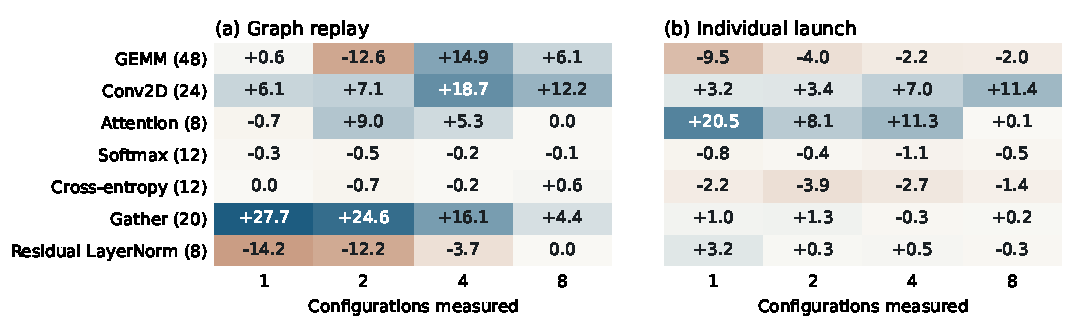
\includegraphics[width=\textwidth]{portfolio_budgets.pdf}
\caption{Five-GPU independent-pass success rate of the adaptive Gaussian surrogate minus that of the shape-conditioned fixed portfolio (percentage points). Blue favors the adaptive policy and orange favors the portfolio. Parentheses give the number of candidates per task. Each cell averages over held-out shapes, precisions and eligible GPUs. Both policies return the fastest configuration measured on the selection pass.}
\label{fig:portfolio}
\end{figure*}

\begin{table*}[!t]
\centering
\caption{Original four-GPU search and latency prediction. $S_4$ is success after four
evaluations, and $B_{90}$ is the evaluation budget for 90\% success in each
family. Predictions use a common set of four measurements. All entries
other than budgets are percentages. The feedback ablation and random search
are selection controls.}
\label{tab:main}
\small
\setlength{\tabcolsep}{6pt}
\begin{tabular}{lrrrrrrrr}
\toprule
 & \multicolumn{4}{c}{Graph replay} & \multicolumn{4}{c}{Individual launch} \\
\cmidrule(lr){2-5}\cmidrule(lr){6-9}
Method & $S_4$ & $B_{90}$ & MAPE & Within 10\% & $S_4$ & $B_{90}$ & MAPE & Within 10\% \\
\midrule
Gaussian surrogate & 93.7 & 6 & 17.8 & 46.0 & 72.7 & 14 & 25.8 & 39.4 \\
Geometry ridge & 93.6 & 6 & 18.0 & 45.6 & 72.9 & 15 & 25.7 & 39.4 \\
Ranked FiLM & 87.1 & 11 & 20.9 & 34.8 & 72.3 & 14 & 25.1 & 42.5 \\
Boosted tree & 88.3 & 16 & 24.5 & 34.4 & 68.1 & 17 & 29.9 & 28.4 \\
Target-only GP--EI & 84.7 & 12 & 20.4 & 42.8 & 72.5 & 16 & 35.6 & 40.3 \\
Gaussian, no feedback & 85.4 & 9 & -- & -- & 72.4 & 15 & -- & -- \\
Gaussian, offset-only forecast & -- & -- & 20.6 & 39.7 & -- & -- & 25.2 & 42.7 \\
Random search & 64.7 & 32 & -- & -- & 66.5 & 28 & -- & -- \\
\bottomrule
\end{tabular}

\end{table*}



\section{Evaluation}
\subsection{Matched GPU measurements}
The benchmark covers GEMM, Conv2D, attention, softmax, cross-entropy,
gather, and residual layer normalization. The original four-GPU study
used 60,000 FP16 device--configuration pairs on H100, RTX 3070 (WSL),
RTX A5000, and T4, and 45,000 BF16 pairs on the first three devices.
H100 and RTX 3070 labels aggregate three passes, A5000 and T4 one.
The Colab T4 used PyTorch 2.6 and Triton 3.2, the others PyTorch 2.8
and Triton 3.4. T4 transfer therefore also changes the software stack.
All scored candidates passed correctness checks in both timing modes.

We report median CUDA-event times over 50 samples per configuration,
pass, and mode. After a 0.1-s workload warm-up, individual samples time
one launch and synchronize on its end event. Graph capture and pilot
runs precede measurement. Graph samples time one replay and divide by its captured
launch count (8, 32, 128, 512, or 2,048), increased until the pilot
median reaches 0.75 ms or the cap. We counterbalance mode order and
check outputs before and after timing. The native A100 uses this same
timer after a separate stability pilot.

Each fold holds out a GPU and either the largest or next-largest shapes
(199 shapes per range). Source training and validation exclude the
held-out GPU and shapes. The original evaluation scores 2,786
device--shape--precision cases and 41,888 candidate timings per mode.
Adding the native A100 and independent passes yields 405,000 rows from
three passes over 75,000 FP16 and 60,000 BF16 device--configuration
pairs, each with both timing medians.

\subsection{Comparators}
\textbf{Fixed portfolios} greedily add the configuration that covers the
most additional source tasks within 5\% of their best latency. Each
prefix defines a fixed set for budgets 1, 2, 4, and 8. The global
portfolio uses the training shapes in the current family, precision,
timing mode, and fold. The local portfolio uses
the eight nearest training shapes per source GPU (scaled log dimensions
and a gather-locality mismatch penalty). Ties favor lower mean best log
slowdown, then candidate index. Both choose the full list before observing
any target latency. After timing the list, each returns its fastest
measured member.

\textbf{Geometry ridge} uses the same source prediction and residual
covariance as the belief-state surrogate. Its first timing anchors absolute
scale, and subsequent timings update log-latency contrasts relative to that
anchor. This is the closest comparison.

\textbf{Ranked FiLM}~\cite{film} predicts a source-trained within-workload ordering.
Hardware descriptors modulate the network's workload and configuration
features. The ranking determines a fixed evaluation order. A source-validation
monotone calibration maps ranks to relative log latency, followed by target
scale calibration for the prediction comparison.

\textbf{Boosted tree} ranks candidates by source-trained log latency;
four common target timings calibrate its prediction offset.
\textbf{Target-only GP--EI} starts with two charged space-filling
queries, then applies expected improvement with a candidate-geometry
kernel. It differs from the Gaussian surrogate in prior, kernel and
initialization. \textbf{Random search} gives the exact expected success
of uniform sampling without replacement.

\subsection{Budgets, metrics, and uncertainty}
In offline replay, a policy receives the measured latency when it
evaluates a configuration. Let $I_B$ denote the configurations evaluated
within budget $B$ and $t^*$ the minimum measured latency in the task's
search space. Simple regret is
\begin{equation}
 r_B = \frac{\min_{c\in I_B}t_c}{t^*}-1 .
\end{equation}
For independent passes $p$ and $q$, we keep the winner
$c_p=\arg\min_{c\in I_B}t_{p,c}$ (earliest query breaks ties) and score
$r_{B,p\to q}=t_{q,c_p}/\min_{c\in\mathcal C} t_{q,c}-1$.
We report $S_B$, the fraction of tasks with $r_B\leq0.05$, and $B_{90}$,
the smallest budget for which $S_B\geq0.90$ in every kernel family.
Each evaluation counts one distinct configuration, up to the size of the
search space. The replay measures evaluation counts. End-to-end tuning
time also includes compilation, correctness checks, and search overhead.

For prediction, every method receives the first four measurements from
the archived hardware-feature adaptive ridge policy. We report mean
absolute percentage error (MAPE) and the fraction of predictions within
10\% of measured latency on configurations outside those four.

We average prediction errors over configurations within a task. Then we
weight kernel families, precisions, and held-out size ranges equally.
Available GPUs receive equal weight within each shape and precision.
We obtain 95\% pointwise intervals from 10,000 paired bootstrap samples of whole
shapes within each family and size range, retaining all device and
precision observations of each sampled shape.

\section{Results}
\subsection{Configuration search}
On the original four GPUs, same-pass feedback raises four-probe
graph-replay success from 85.38\%
to 93.66\%. GEMM rises from 48.47\% to 81.67\% and Conv2D from 70.63\%
to 92.06\%. Together they account for 94\% of
the net gain under equal family weights. Softmax already succeeds on
99.33\% of tasks with feedback disabled. Individual-launch success
changes from 72.39\% to 72.74\%. The graph-minus-individual difference
in feedback gains is 7.93 percentage points (paired 95\% interval
$[5.95,9.94]$).

Adaptive geometry ridge and the Gaussian surrogate both reach $B_{90}$ at
six graph evaluations. Individual launches require fifteen for ridge and
fourteen for Gaussian (Table~\ref{tab:main}).
The four-evaluation Gaussian-minus-ridge differences are
$\GraphRidgeDelta$ points ($\GraphRidgeCI$) and $\LaunchRidgeDelta$
($\LaunchRidgeCI$), respectively.

\subsection{Does the selected configuration stay fast?}
We replay each policy using timings from one pass and score its selected
configuration against the fastest candidate on a different pass. The
same 1,000 FP16 workloads span all five environments. Four also support
the 1,000 BF16 workloads. We retain the original source fits for H100,
RTX 3070, A5000, and T4. The A5000 repeat passes use one board distinct
from the original A5000. For the native A100 we fit on the original
non-A100 sources and exclude the test shapes. Each policy is scored on
796 held-out cases per timing mode on each BF16-capable GPU and 398 on
T4. On each GPU, three passes give six ordered pairs for selection and
scoring. We average these pairs within each case before resampling shapes.

Feedback improves graph-replay success by 3.84 to 9.72 percentage
points across GPUs (Table~\ref{tab:passes}). Its effect is smaller for
individual launches, where Gaussian success ranges from 20.9\% on RTX
3070 to 87.1\% on A100. Gaussian and ridge success rates differ by less
than half a point in every device and timing mode.

\begin{table}[t]
\centering
\caption{Five-GPU independent-pass success (\%) after four evaluations. On and
Off denote the Gaussian surrogate with measured feedback enabled and
disabled. Ridge uses adaptive geometry ridge.}
\label{tab:passes}
\footnotesize\setlength{\tabcolsep}{3pt}
\begin{tabular}{lrrrrrr}
\toprule
 & \multicolumn{3}{c}{Graph replay} & \multicolumn{3}{c}{Individual launch} \\
\cmidrule(lr){2-4}\cmidrule(lr){5-7}
GPU & On & Off & Ridge & On & Off & Ridge \\
\midrule
H100 & 93.1 & 83.3 & 93.1 & 84.0 & 85.8 & 83.9 \\
A100 & 81.6 & 77.7 & 81.5 & 87.1 & 87.6 & 87.1 \\
A5000 & 91.8 & 83.4 & 91.8 & 65.4 & 62.8 & 65.4 \\
3070 (WSL) & 86.9 & 83.0 & 87.3 & 20.9 & 20.7 & 20.9 \\
T4 & 83.9 & 77.5 & 84.0 & 38.1 & 37.7 & 38.2 \\
\bottomrule
\end{tabular}

\end{table}

\subsection{Can a fixed shortlist recover the gain?}
With four graph evaluations the Gaussian policy succeeds on 87.9\% of
cases, compared with 77.6\% for the global and 80.7\% for the local
portfolio (Table~\ref{tab:portfolio}). The local gap peaks at four
probes among the budgets tested. Four of 48 GEMM candidates give
a 14.9-point advantage over the local portfolio, while four of eight
residual layer normalization candidates favor the portfolio by 3.7 points
(Fig.~\ref{fig:portfolio}). On RTX 3070 the graph difference is
$-1.7$ points (95\% interval $[-4.5,1.3]$).

On individual launches the four-probe gain over the global portfolio is
0.7 points $[-0.2,1.5]$. A portfolio comparison also changes the initial ranking.
For gather, the Gaussian policy gains 16.1 points over the local
portfolio but just 0.3 over its own feedback-disabled policy. The
matched feedback gains are 26.7 points for GEMM and 19.1 for Conv2D.
Across families, feedback adds 6.70 points $[5.22,8.18]$ in graph
replay and 0.08 $[-0.41,0.56]$ for individual launches. At one probe
the two Gaussian policies always choose the same candidate.

\begin{table}[t]
\centering
\caption{Five-GPU independent-pass success (\%). Global and Local are
fixed portfolios. The paired difference (points) compares Gaussian with
Local. Each budget measures distinct configurations.}
\label{tab:portfolio}
\footnotesize\setlength{\tabcolsep}{3pt}
\begin{tabular}{lrrrrr}
\toprule
Mode & $B$ & Gaussian & Global & Local & $\Delta_{\rm local}$ [95\% CI] \\
\midrule
Graph & 1 & 58.7 & 48.4 & 55.9 & +2.7 [+0.4, +5.1] \\
 & 2 & 69.8 & 60.4 & 67.7 & +2.1 [-0.3, +4.6] \\
 & 4 & 87.9 & 77.6 & 80.7 & +7.3 [+5.5, +9.0] \\
 & 8 & 92.0 & 87.5 & 88.7 & +3.3 [+2.3, +4.3] \\
\midrule
Individual & 1 & 51.7 & 53.2 & 49.5 & +2.2 [+0.9, +3.5] \\
 & 2 & 55.8 & 55.6 & 55.1 & +0.7 [-0.5, +1.9] \\
 & 4 & 61.4 & 60.7 & 59.6 & +1.8 [+0.7, +2.8] \\
 & 8 & 64.6 & 63.4 & 63.5 & +1.1 [+0.2, +1.9] \\
\bottomrule
\end{tabular}

\end{table}

\subsection{Latency prediction}
With the same four measurements, the Gaussian surrogate's MAPE is 17.8\%
on graph replay and 25.8\% on individual launches (Table~\ref{tab:main}).
The fractions of predictions within 10\% of measured latency are 46.0\%
and 39.4\%. Ranked FiLM achieves 25.1\% MAPE on individual launches at
the same $B_{90}$ of fourteen. A simpler forecast adds the median
observed log-latency offset to every source prediction. Its MAPE is
\GraphOffsetMAPE\% on graph replay and \LaunchOffsetMAPE\% on individual
launches. Updating correlated configurations helps prediction under the
first protocol and increases mean error under the second.

\section{Limitations}
Our evaluation covers fixed Triton templates and configurations that pass
correctness checks. Timing protocols, software stacks, and measurement
repetitions vary across GPU environments. The intervals condition on
the measured environments. We explored surrogate variants on these benchmark ranges before choosing
the Gaussian model. Independent-pass scoring tests timing repeatability on the same tasks. We retained the original source fits and acquisition rules for the four original targets.
The native A100 supplies a held-out device with the same kernel templates.
Transfer to new templates remains open.

Repeated measurements can change the ordering of configurations. On RTX 3070, selecting the fastest
FP16 configuration in one pass and scoring it on another gives 86.2\%
success under graph replay and 19.2\% under individual launches.
Graph replay changes both execution and timing granularity. These measurements cannot separate those effects or establish a wall-clock tuning advantage.

\section{Conclusion}
At four probes the adaptive Gaussian surrogate beats both fixed
portfolios on average for graph replay. The matched ablation attributes
most of the feedback benefit to GEMM and Conv2D. Individual launches
show little average benefit from feedback, and adaptive geometry ridge
achieves similar success across both protocols.

\noindent\textit{Artifact.} The replication package includes collectors,
selection traces, and workload-by-budget results. Run
\texttt{make portfolio} to replay the fixed and adaptive policies.

\section*{Acknowledgments}
We thank the Texas Advanced Computing Center (TACC) at The University of
Texas at Austin for providing the Lonestar6 resources used for the A100
and H100 measurements.

\section*{Use of AI tools}
OpenAI Codex assisted with literature search, benchmark implementation,
analysis, and drafting.

\bibliographystyle{IEEEtran}
\bibliography{references}
\end{document}
